\documentclass{article}

\usepackage{graphicx}
\usepackage{amsmath,amssymb,amsfonts,amsthm,mathtools} % Mathematik
\usepackage{subfigure} 
\usepackage{color}

\usepackage{pdfpages}

\usepackage[top=1.5cm, bottom=1.5cm]{geometry}

\title{Sheet 3 - Answers}
\author{Timm \& Boris}

\begin{document}
\maketitle

\section*{Task: 1}

Wird vielleicht noch nachgereicht, falls ich den Beweis noch hinkriege.\\
Momentaner Ansatz befindet sich im Ordner BaSheet03/Task01.

{\textit{Timm}}

\section*{Task: 3}
% 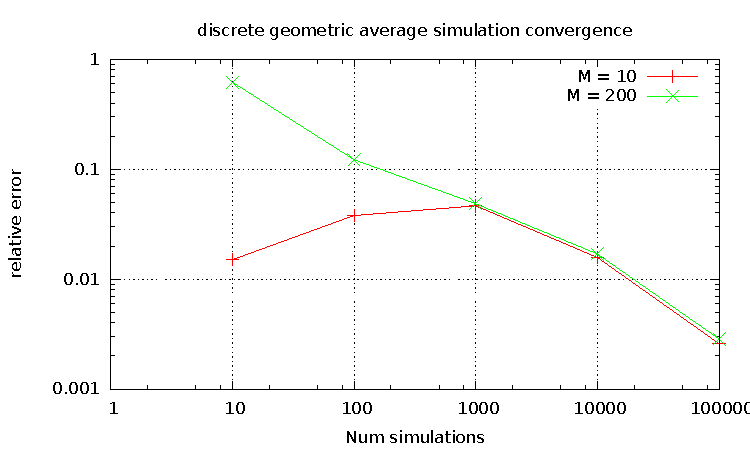
\includepdf{../Task03/sh3_task3_convergence_plot.pdf}
The Plot illustrates the convergence of payout simulations from discrete geometric Asian options.
After plotting some simulations, we get the result that the convergence for M=10 and M=200 behaves similar. There was no clear advantage of either. Example:\\
\begin{figure}[htbp]
  \centering
     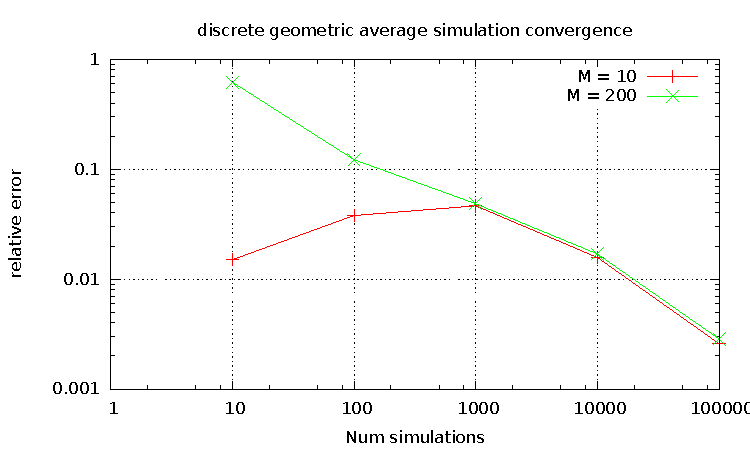
\includegraphics[width=1.0\textwidth]{../Task03/sh3_task3_convergence_plot.pdf}
%    \caption{}
\end{figure}
\newpage

\section*{Task: 4}
This Task illustrates the convergence of discrete geometric to continuous geometric (closed solutions for Asian fair price). We observe a linear graph in a log log plot that has the slope 1, what means that the convergence is polynomial with rate 1.
\begin{figure}[htbp]
  \centering
     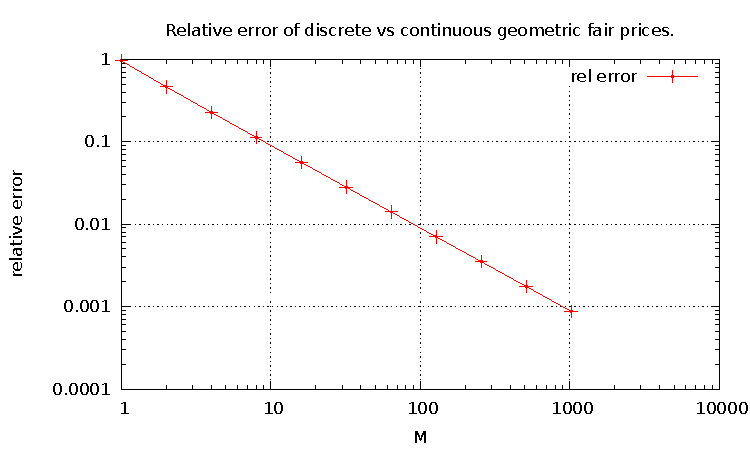
\includegraphics[width=1.0\textwidth]{../Task04/sh3_task4_convergence_plot.pdf}
%    \caption{}
\end{figure}

\section*{Task: 5}
This is a Plot of the integrand of the discrete arithmetic average for M = 2.
\begin{figure}[htbp]
  \centering
     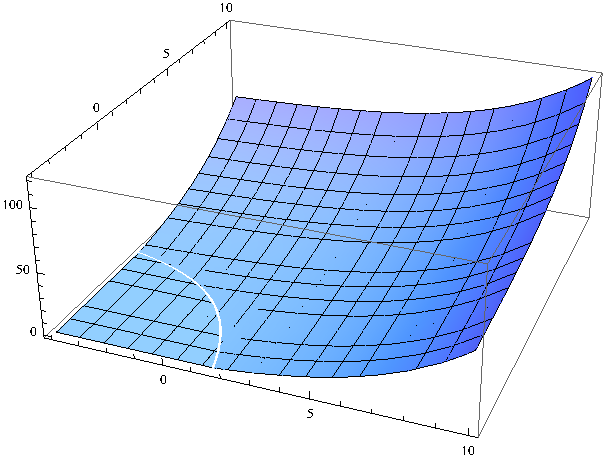
\includegraphics[width=0.8\textwidth]{../Task05/sh3_task5_arithmetic_payoff.pdf}
%    \caption{}
\end{figure}

\newpage
\section*{Task: 7}
Here are the Points of the first 100 Halton points from task 6 compared with uniform ones.
\begin{figure}[htbp]
  \centering
     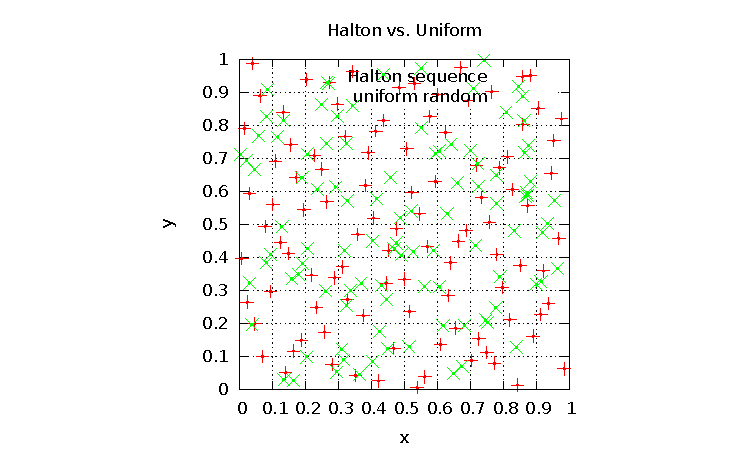
\includegraphics[width=1.0\textwidth]{../Task07/sh3_task7_point_plot.pdf}
%    \caption{}
\end{figure}

\section*{Task: 9}
\begin{figure}[htbp]
  \centering
     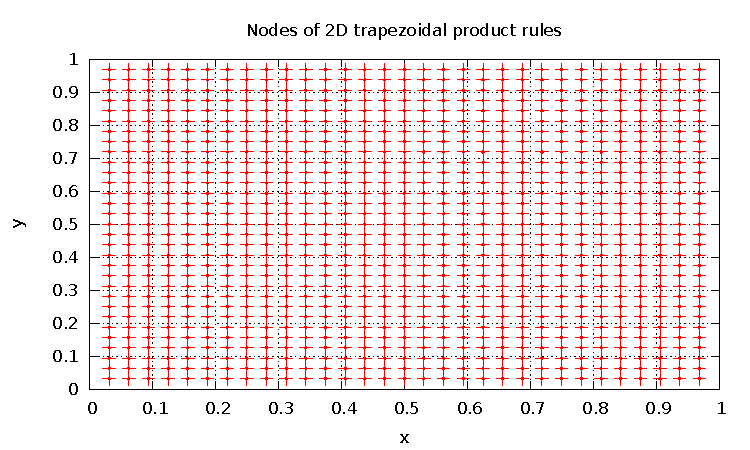
\includegraphics[width=1.0\textwidth]{../Task09/sh3_task9_point_plot_trapezoidal.pdf}
%    \caption{}
\end{figure}
\newpage
\begin{figure}[htbp]
  \centering
     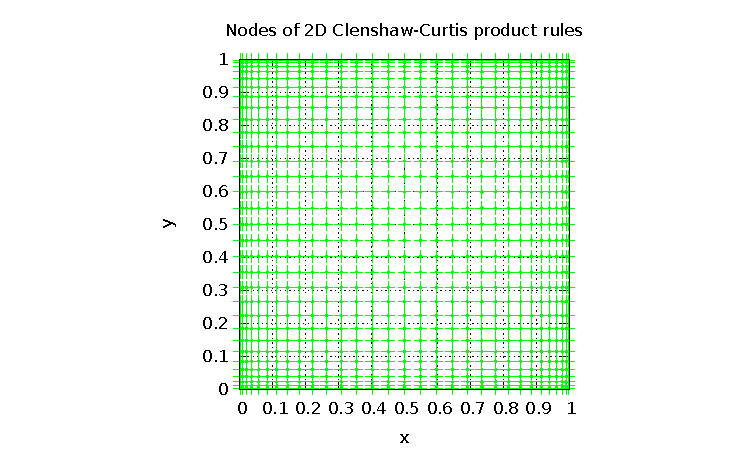
\includegraphics[width=1.0\textwidth]{../Task09/sh3_task9_point_plot_clenshawCurtis.pdf}
%    \caption{}
\end{figure}

\begin{figure}[htbp]
  \centering
     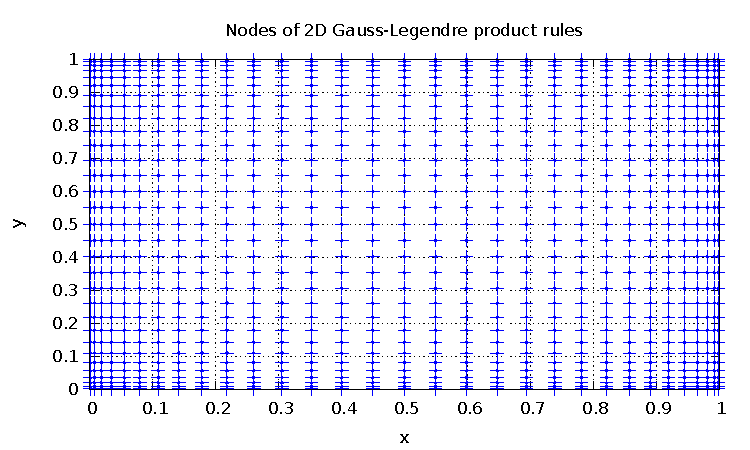
\includegraphics[width=1.0\textwidth]{../Task09/sh3_task9_point_plot_gaussLegendre.pdf}
%    \caption{}
\end{figure}

\newpage
\section*{Task: 11}
\begin{figure}[htbp]
  \centering
     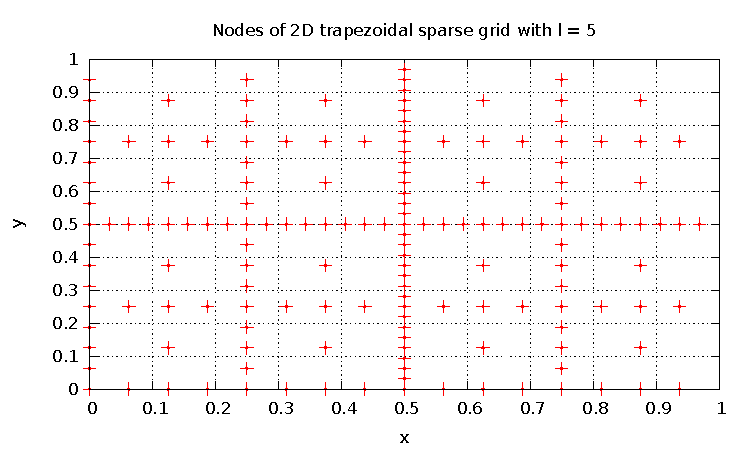
\includegraphics[width=1.0\textwidth]{../Task11/sh3_task11_point_plot_trapezoidal_l=5.pdf}
%    \caption{}
\end{figure}

\begin{figure}[htbp]
  \centering
     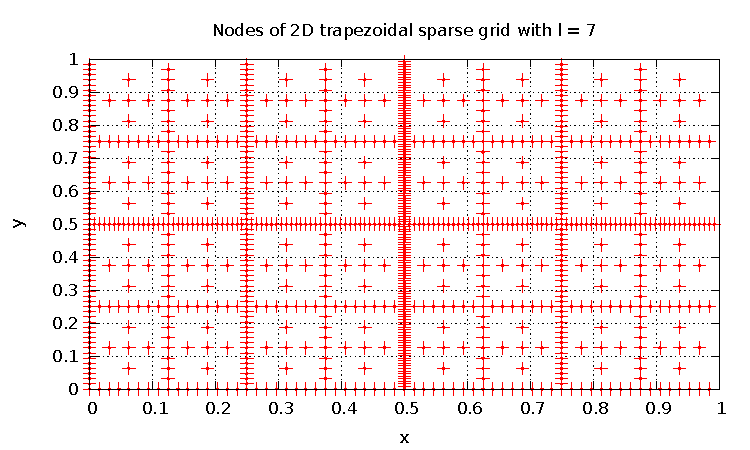
\includegraphics[width=1.0\textwidth]{../Task11/sh3_task11_point_plot_trapezoidal_l=7.pdf}
%    \caption{}
\end{figure}
\newpage
\begin{figure}[htbp]
  \centering
     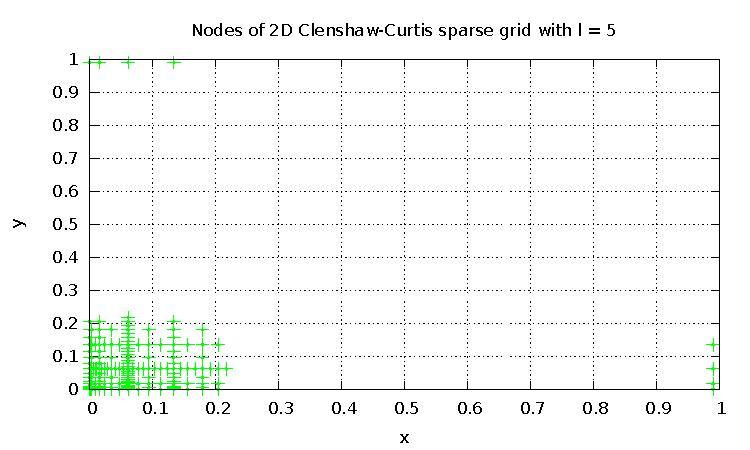
\includegraphics[width=1.0\textwidth]{../Task11/sh3_task11_point_plot_clenshawCurtis_l=5.pdf}
%    \caption{}
\end{figure}

\begin{figure}[htbp]
  \centering
     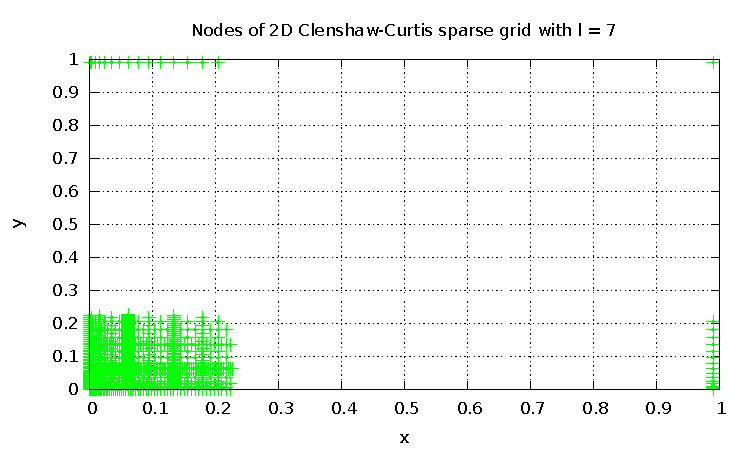
\includegraphics[width=1.0\textwidth]{../Task11/sh3_task11_point_plot_clenshawCurtis_l=7.pdf}
%    \caption{}
\end{figure}

\newpage
\section*{Task: 12}
Plot of the number of Points of sparse and product grid.
\begin{figure}[htbp]
  \centering
     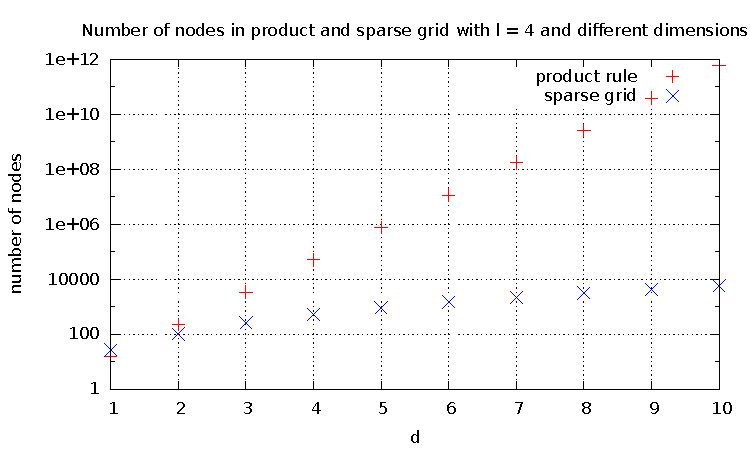
\includegraphics[width=1.0\textwidth]{../Task12/sh3_task12_num_of_nodes.pdf}
%    \caption{}
\end{figure}

\section*{Task: 13}
Here is a convergence plot for the function: 
\[ f_{\gamma}(x_1, \dots , x_d) = \prod_{j=1}^{d} f_{\gamma}(x_j) =  \prod_{j=1}^{d} \left(1 + \gamma e^{\frac{x_j}{2}}\right) \]
with our known integration methods.
\begin{figure}[htbp]
  \centering
     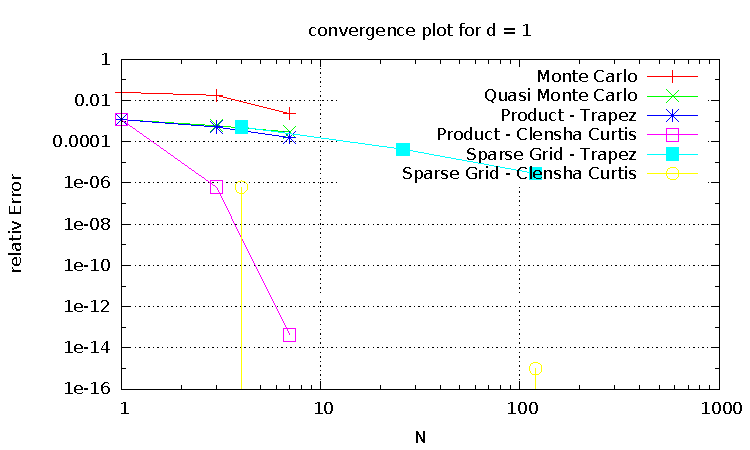
\includegraphics[width=1.0\textwidth]{../Task13/sh3_task13_convergencePlotd1.pdf}
%    \caption{}
\end{figure}
\newpage
\begin{figure}[htbp]
  \centering
     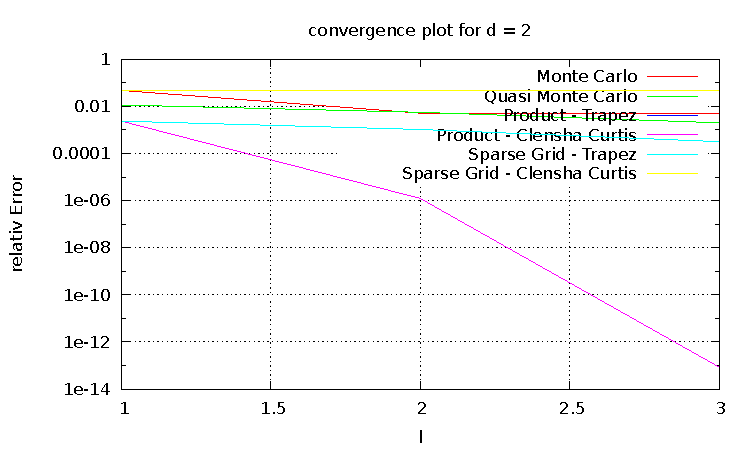
\includegraphics[width=1.0\textwidth]{../Task13/sh3_task13_convergencePlotd2.pdf}
%    \caption{}
\end{figure}

\begin{figure}[htbp]
  \centering
     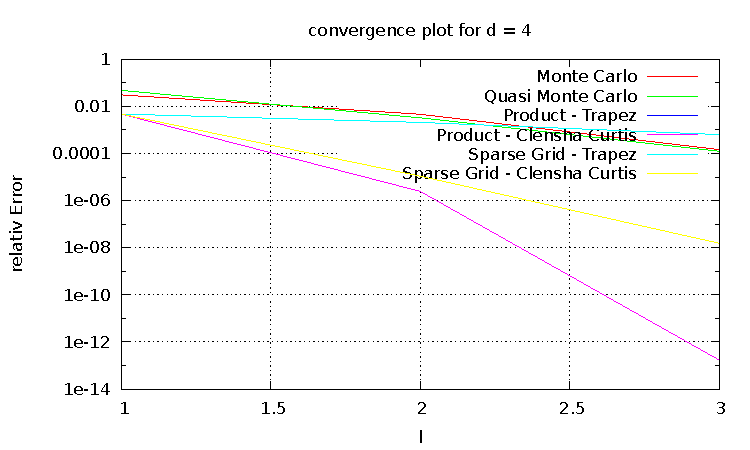
\includegraphics[width=1.0\textwidth]{../Task13/sh3_task13_convergencePlotd4.pdf}
%    \caption{}
\end{figure}
\newpage
\begin{figure}[htbp]
  \centering
     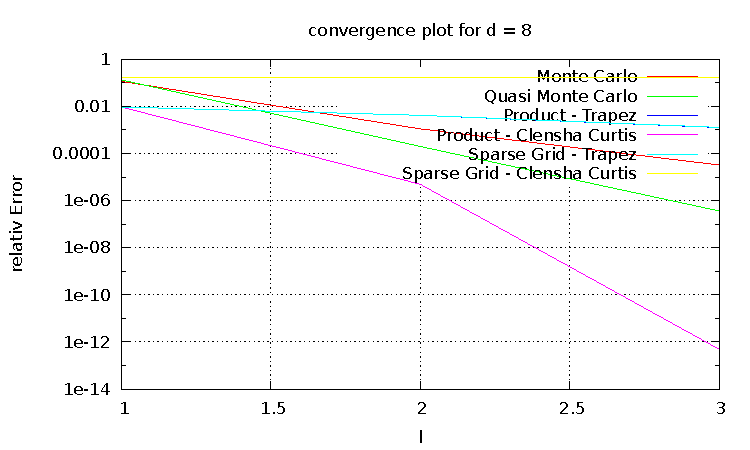
\includegraphics[width=1.0\textwidth]{../Task13/sh3_task13_convergencePlotd8.pdf}
%    \caption{}
\end{figure}

\section*{Task: 15}
We integrated the discrete geometric Asian option for Brownian bridge and Random walk constructions with Cleshaw Curtis sparse grid. The observation was that for level 4 we get the same value  10.4889 with an error of Order $ O(10^{-5}) $.

\newpage
\section*{Task: 16}
All integration methods we know applied to task 15.
% \begin{figure} [htbp]
% 	\begin{minipage}[b]{0.5\textwidth} 
%     	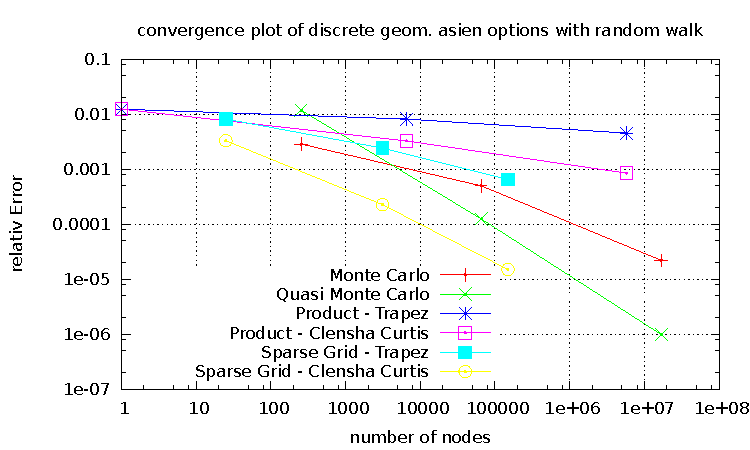
\includegraphics[width=1\textwidth]{../Task16/sh3_task16_convergence_plot_rw.pdf}
%     \end{minipage}
%     \begin{minipage}[b]{0.5\textwidth} 
%     	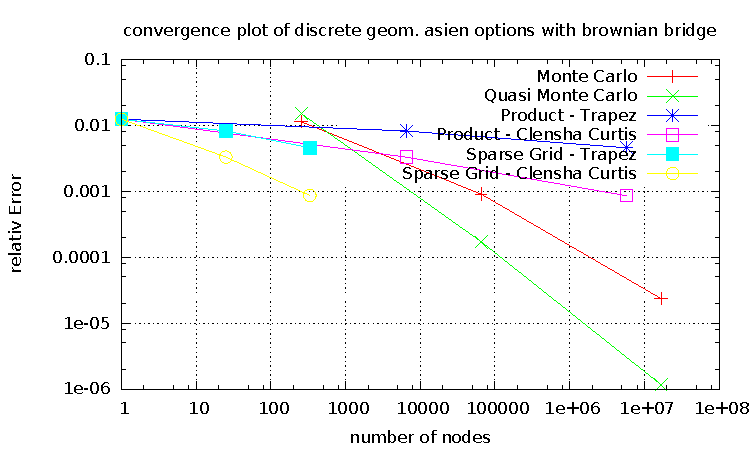
\includegraphics[width=1\textwidth]{../Task16/sh3_task16_convergence_plot_bb.pdf}
%     \end{minipage}
% \caption{Plots of Task 5} 
% \end{figure} 
\begin{figure}[htbp]
 \centering
    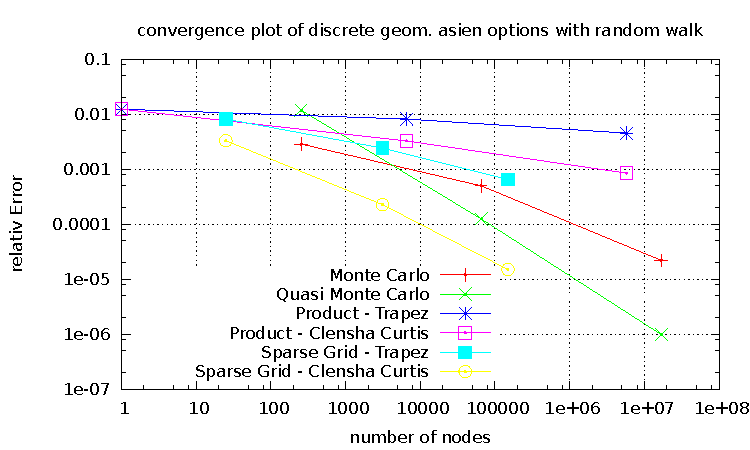
\includegraphics[width=1.0\textwidth]{../Task16/sh3_task16_convergence_plot_rw.pdf}
%    \caption{}
\end{figure}

\begin{figure}[htbp]
 \centering
    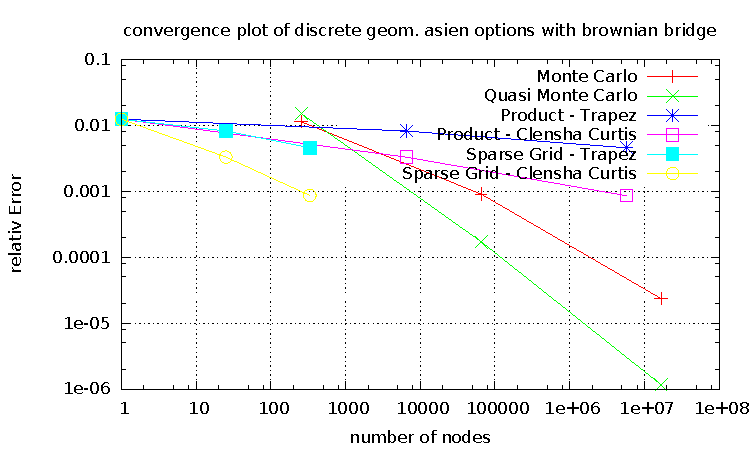
\includegraphics[width=1.0\textwidth]{../Task16/sh3_task16_convergence_plot_bb.pdf}
%    \caption{}
\end{figure}

\newpage

\section*{Task: 17}
This is also a convergence plot for the discrete geometric Asian option with Brownian bridge and Random walk. Both with Monte Carlo and Quasi Monte Carlo.
\begin{figure}[htbp]
  \centering
     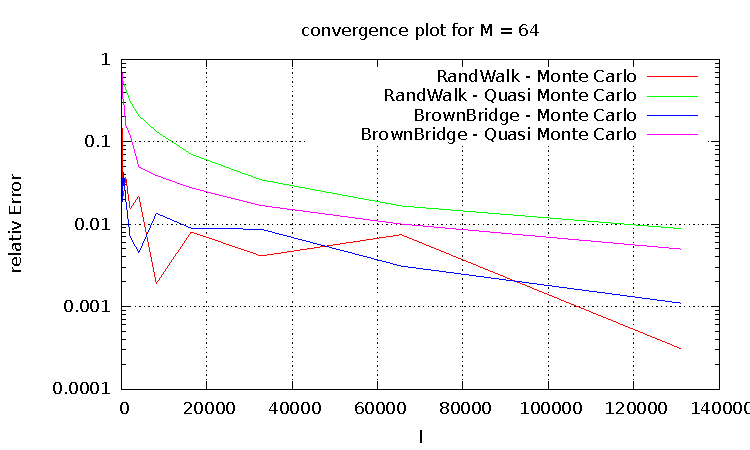
\includegraphics[width=1.0\textwidth]{../Task17/sh3_task17_convergencePlot.pdf}
%    \caption{}
\end{figure}

\section*{Task: 18}

Because of the impact of the dimension into the convergence rate, 
the product rule should be used for low dimensions, 
the sparse grid can be used for higher dimensions, then quasi Monte Carlo and
for any high dimension the Monte Carlo integration method whichs convergence rate does not depend on the dimension. 

\end{document}